\documentclass[12pt]{article}
\usepackage[margin=1in]{geometry}
\usepackage{amsmath,amssymb,amsthm,booktabs,graphicx,natbib,microtype,array}
\newtheorem{theorem}{Theorem}
\newtheorem{corollary}[theorem]{Corollary}
\newtheorem{proposition}[theorem]{Proposition}
\newtheorem{remark}[theorem]{Remark}
\title{A Correlated Base--Tail Viability Tube\\\large Signed Support Cocycles beyond Unsigned Projective Products}
\author{Prime Dynamics Theory Program}
\date{July 2026}

\begin{document}
\maketitle

\begin{abstract}
The directional candidate is the product
\[
 S(y,a)=a(1-\sqrt y)_+^4,
 \]
where $y$ is a controlled upper for the squared relative tail and
$a\in(0,1]$ is a normalized Gram base.  Previous layers bounded the two
factors separately.  We instead study the correlated support tube
\[
 \mathcal K_\beta=\{(y,a):S(y,a)\geq\beta\}.
\]
If a transition satisfies $y'\leq F(y)$ and $a'\geq r a$, then its sharp
tube multiplier is
\[
 \kappa(y)=r\frac{(1-\sqrt{F(y)})_+^4}{(1-\sqrt y)^4},
 \qquad S(y',a')\geq\kappa(y)S(y,a).
\]
A positive support floor follows whenever the partial sums of
$\log\kappa_n$ are uniformly bounded below.  This signed-cocycle condition
allows losses followed by recoveries and is therefore more flexible than
summability of the unsigned projective distances in RH-146.  It is sharp for
the stated transition information: if the partial sums diverge to
$-\infty$, the equality trajectory has zero support liminf.

The outward RH-138 archive contains 328 positive states and 28/30 complete
chains in the common tube $\mathcal K_{10^{-10}}$.  The delayed clean suffix
from $\sigma=0.04$ contains 18/18 chains in a common tube above
$1.5\times10^{-10}$.  Local support multipliers include 98 recoveries above
one and 194 losses below one.  Direct statewise reanchoring improves the
RH-146 projective product by between $1.35\times10^{16}$ and
$4.44\times10^{48}$.  These are finite correlated certificates; no
all-level support cocycle or cross-scale reset is proved.
\end{abstract}

\section{Why a joint tube}
Write
\[
 \phi(y)=(1-\sqrt y)_+^4,
 \qquad S(y,a)=a\phi(y).
\]
RH-139 uses the sufficient conditions $\limsup y_n<1$ and
$\liminf a_n>0$.  RH-146 gives a sharp projective recurrence for $a_n$, but
its unsigned product loses 16--49 orders of magnitude on the finite chains.
The loss is structural: every step is charged its worst possible shape
distortion even if a later transition repairs it.

The superlevel set $\mathcal K_\beta$ keeps the two factors at their common
time index.  It is not a logically weaker asymptotic goal.  Because
$0<a\leq1$ and $0\leq\phi\leq1$,
\begin{equation}\label{eq:implications}
 S(y,a)\geq\beta
 \quad\Longrightarrow\quad
 a\geq\beta,
 \qquad
 y\leq(1-\beta^{1/4})^2<1.
\end{equation}
Conversely, $y\leq\bar y<1$ and $a\geq a_*>0$ imply
$S(y,a)\geq a_*\phi(\bar y)$.  Thus a positive eventual joint tube is
equivalent in qualitative force to the two RH-139 packets, while permitting
a proof to preserve levelwise correlation.

\section{Sharp tube transport}
Suppose an available control gives a monotone tail upper $F$ and a lower
base ratio $r>0$:
\begin{equation}\label{eq:transition}
 y'\leq F(y),
 \qquad
 a'\geq r a.
\end{equation}
The base ratio may come from a direct Gram comparison, an interval enclosure,
or a block estimate.  The theorem itself is independent of its source.

\begin{theorem}[Sharp correlated multiplier]\label{thm:multiplier}
For every source state with $0\leq y<1$, transition
\eqref{eq:transition} implies
\begin{equation}\label{eq:multiplier}
 S(y',a')\geq \kappa(y)S(y,a),
 \qquad
 \kappa(y)=r\frac{\phi(F(y))}{\phi(y)}.
\end{equation}
This multiplier is sharp given only \eqref{eq:transition}.
\end{theorem}
\begin{proof}
The function $\phi$ is decreasing.  Hence
\[
 S(y',a')=a'\phi(y')
 \geq ra\phi(F(y))
 =r\frac{\phi(F(y))}{\phi(y)}S(y,a).
\]
Equality occurs when $y'=F(y)$ and $a'=ra$, so no larger universal
multiplier follows from the two scalar bounds alone.
\end{proof}

\begin{corollary}[One-step tube invariance]
On a source-tail domain $I\subset[0,1)$, the information
\eqref{eq:transition} preserves every tube $\mathcal K_\beta$ if
\[
 \inf_{y\in I}\kappa(y)\geq1.
\]
For the stated information set this criterion is exact: if it fails at
$y_0$, the extremal boundary state
$a=\beta/\phi(y_0)$ exits $\mathcal K_\beta$ under equality in
\eqref{eq:transition}.
\end{corollary}

If $F(y)\geq1$, the target factor vanishes and no positive tube can pass that
state.  The superunit birth obstruction of RH-144--RH-145 is therefore
recovered automatically in the joint geometry.

\section{Signed support cocycles}
One-step invariance is stronger than necessary.  A lossy step can be crossed
if later recoveries prevent the cumulative product from approaching zero.

\begin{theorem}[Lower-bounded logarithmic cocycle]\label{thm:cocycle}
Suppose a controlled trajectory obeys
\[
 S_{n+1}\geq\kappa_nS_n,
 \qquad \kappa_n>0,
\]
for $n\geq N$.  If there is $C<\infty$ such that
\begin{equation}\label{eq:partial}
 \sum_{j=N}^{n-1}\log\kappa_j\geq-C
 \quad\text{for every }n>N,
\end{equation}
then
\[
 \inf_{n\geq N}S_n\geq S_Ne^{-C}>0.
\]
Consequently both conclusions in \eqref{eq:implications} hold eventually.
\end{theorem}
\begin{proof}
Iteration gives
$S_n\geq S_N\exp(\sum_{j=N}^{n-1}\log\kappa_j)$, and
\eqref{eq:partial} gives the stated floor.
\end{proof}

The condition keeps signs.  Infinitely many $\kappa_n<1$ are harmless when
they are offset by sufficiently strong $\kappa_n>1$ steps.  This differs
from the RH-146 sufficient condition $\sum d_n<\infty$, which charges every
projective movement positively.

\begin{proposition}[Sharp cocycle obstruction]\label{prop:sharp}
If the partial logarithmic sums are unbounded below, no positive universal
support floor follows from the multiplier sequence alone.
\end{proposition}
\begin{proof}
Choose the admissible equality trajectory
$S_{n+1}=\kappa_nS_n$.  Along a subsequence where the partial sums tend to
$-\infty$, this trajectory tends to zero.  The constant sequence
$\kappa_n=1/2$ is the simplest witness.
\end{proof}

For controlled families, one may select $c_n$ and use
\[
 \kappa_{n,c_n}(y_n)
 =r_{n,c_n}\frac{\phi(F_{n,c_n}(y_n))}{\phi(y_n)}.
\]
This is a viability problem on a multiplicative cocycle
\citep{Aubin1991,Strogatz2018}.  A block theorem needs a uniform bound on the
largest within-block drawdown and a lower bound on all partial sums of block
endpoint gains.  It does not require every local multiplier to exceed one.

\section{Outward finite audit}
We combine the independently outward-guarded tail upper and normalized-base
lower already archived in RH-138.  At each target state we recompute
$S=a\phi(y)$; all 330 recomputations agree with the archived support lower.
The two superunit states have $S=0$.  Every other state exceeds
$1.0365\times10^{-10}$, so 28 complete chains lie in
$\mathcal K_{10^{-10}}$.

\begin{table}[t]
\centering
\scriptsize
\begin{tabular}{ccc}
\toprule
tube level $\beta$ & complete chains in $\mathcal K_\beta$ & interpretation\\
\midrule
$10^{-10}$ & $28/30$ & every finite viable chain\\
$10^{-8}$  & $21/30$ & excludes weak coarse directions\\
$10^{-6}$  & $15/30$ & retains intermediate/fine packets\\
$10^{-4}$  & $12/30$ & exactly the two finest anchors\\
\bottomrule
\end{tabular}
\caption{Complete-chain correlated tube levels.}
\label{tab:tubes}
\end{table}

The RH-145 delayed suffix beginning at $\sigma=0.04$ has 18/18 complete
positive chains and common tube level
$1.55426\times10^{-10}$.  This is a finite cofinal-anchor statement, not a
proof that future anchors enter the same tube.

Among consecutive positive archived states there are 292 local support
ratios.  Their range is
\[
 1.9078\times10^{-4}\leq S_{n+1}/S_n\leq14.7601,
\]
with median $0.6011$.  Ninety-eight ratios are recoveries above one and 194
are losses below one.  Thus per-step invariance is visibly false, while the
finite chains still retain a positive common floor.  This is exactly the
regime addressed by Theorem~\ref{thm:cocycle}.

\begin{figure}[t]
\centering
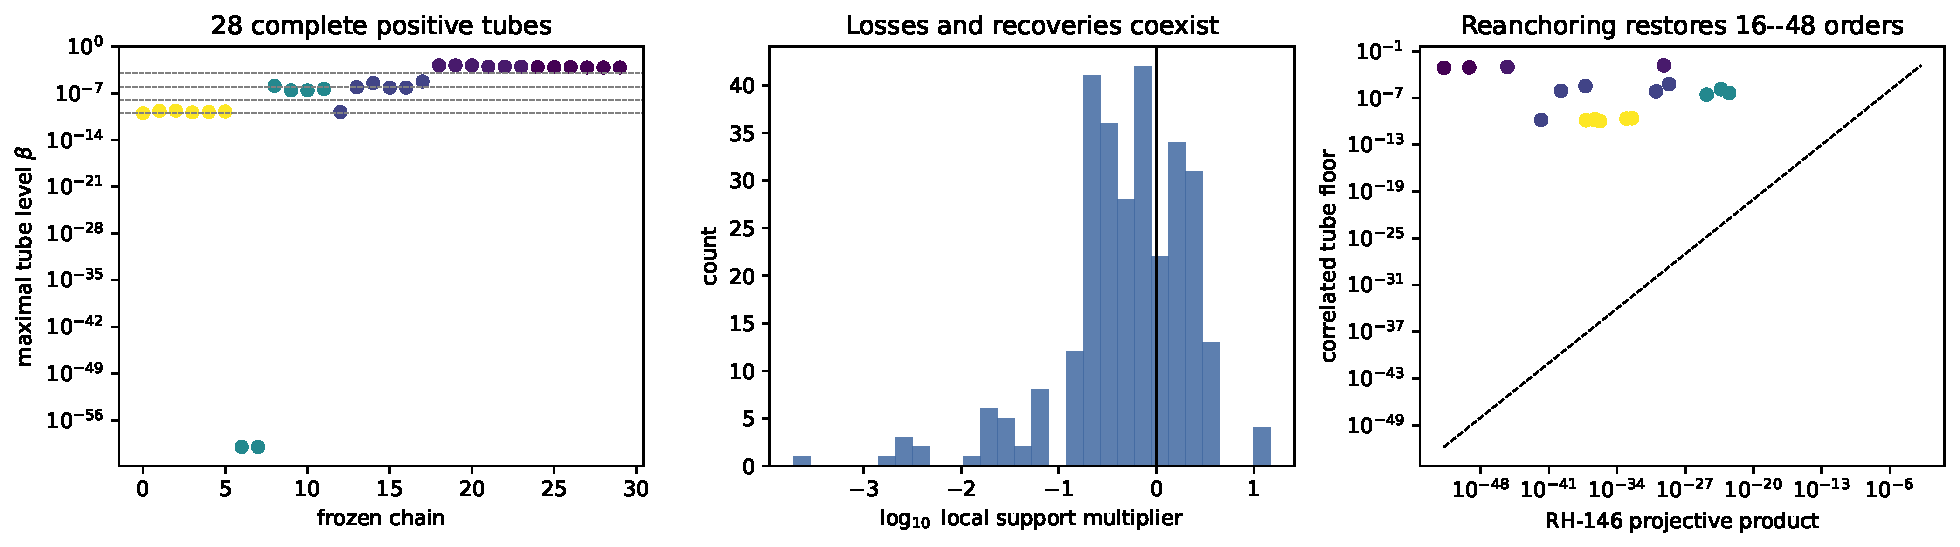
\includegraphics[width=\textwidth]{figures/correlated_base_tail_tube.pdf}
\caption{Finite tube levels, signed local support multipliers, and recovery
relative to the unsigned RH-146 projective product.}
\label{fig:audit}
\end{figure}

The maximum gain from pairing the worst tail and worst base at their actual
common states, rather than as one rectangular chain bound, is only $1.018$.
The major improvement comes from repeated direct reanchoring: relative to the
RH-146 terminal projective products, the correlated tube floors are larger by
$1.35\times10^{16}$ to $4.44\times10^{48}$, with median gain
$3.46\times10^{26}$.  An all-level proof must reproduce this reanchoring or
signed cancellation analytically; finite direct eigenvalue evaluation cannot
substitute for it.

\section{Consequence and claim boundary}
RH-147 replaces two independently propagated worst-case scalars by one exact
support geometry.  The new all-level target is:
\[
 \boxed{\inf_{n\geq N}\sum_{j=N}^{n-1}
 \log\!\left[r_j\frac{\phi(F_j(y_j))}{\phi(y_j)}\right]>-\infty}.
\]
Together with validated source assembly, this single condition yields an
eventual positive directional support floor.  It allows isolated losses,
recoveries, blocks, and delayed start.

The present paper proves the scalar transport and sharp obstruction and
audits a finite outward tube.  It does not construct all-level $F_n$ and
$r_n$ on one interval source path, prove a cross-scale reset, verify a
uniform support cocycle, close Stage A, construct a Hilbert--Polya operator,
identify zeta zeros, or prove the Riemann Hypothesis.

\bibliographystyle{plainnat}
\bibliography{references}
\end{document}

